%dispTree -ll -gg -w -s 85 -t

\documentclass{beamer}
%\usetheme{Madrid}
%\usetheme{Boadilla}
%\usetheme{default}
%\usetheme{Warsaw}
%\usetheme{Bergen}
%\usetheme{Frankfurt}
\usetheme{Darmstadt}

%\usecolortheme{seahorse}
%\usecolortheme{beaver}
\usecolortheme[named=orange]{structure}

\setbeamertemplate{footline}[page number]
%\setbeamercovered{transparent}
\setbeamercovered{invisible}
\setbeamertemplate{navigation symbols}{}

\usepackage{multimedia}
\usepackage{graphicx}
\usepackage[utf8]{inputenc}
%\usepackage[T1]{fontenc}
\usepackage[frenchb]{babel} 
\usepackage[all]{xy}
\usepackage{multirow}
\usepackage{lmodern}
\usepackage{subfigure}
\usepackage{ulem}
\usepackage{hyperref}

%\setbeamertemplate{caption}[numbered] 

%% --------------

\title[Soutenance AI]{Debriefing Année Internationale}
\author{L\'eo B\textsc{audouin}}
\institute[LAAS-CNRS]
{
Replanification en temps réel pour les robots humanoïdes.\\Controle en force d'un bras anthropomorphe.
\\
\medskip
{\emph{leo.baudouin@ifma.fr}}
}
\date{20 janvier 2012}

%% --------------

\begin{document}

%\begin{frame}
%\titlepage
%\end{frame}

\setcounter{page}{14} 

\begin{frame}{Nouvelle Zélande}
\tableofcontents
\end{frame}

\section{Nouvelle Zélande}
\subsection{Présentation}
\begin{frame}{Nouvelle-Zélande}
%\begin{center}
%{\bf Nouvelle Zélande}
%\end{center}
\begin{tabular}{c c}
\begin{minipage}{0.5\linewidth}
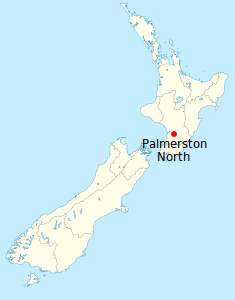
\includegraphics[width=0.9\linewidth]{images/map}
\end{minipage}
&
\begin{minipage}{0.5\linewidth}
\begin{itemize}
\item Palmerston North
\begin{itemize}
\item 210 000 habitants
\item 320 km\up{2}
%\item 758 habitants/km\up{2}
\end{itemize}
\item Culture Anglosaxone / Américaine
\item Santé
\item Accent Néo-Zélandais
\item Coupe de monde de rugby
\end{itemize}
\end{minipage}
\end{tabular}
\end{frame}

%\subsection{Paysages}
%\begin{frame}

%\end{frame}

\subsection{Université}
\begin{frame}{Massey University}
\begin{center}

\includegraphics[width=0.65\linewidth]{images/logo-massey-university}
\begin{itemize}
\item En quelques chiffres
\begin{itemize}
\item 36000 étudiants
\item 3200 emplois
\item 3 campus
\end{itemize}
\vspace{5mm}
%\begin{itemize}
\item \'Equipe de recherche
\begin{itemize}
\item 5 chercheurs
\item 12 étudiants
\item 5 projets
\end{itemize}
\end{itemize}
\end{center}
\end{frame}

\section{Junior}
\subsection{Robot domestique}

\begin{frame}
\begin{center}

\begin{tabular}{c c}
\begin{minipage}{0.4\linewidth}
\begin{figure}
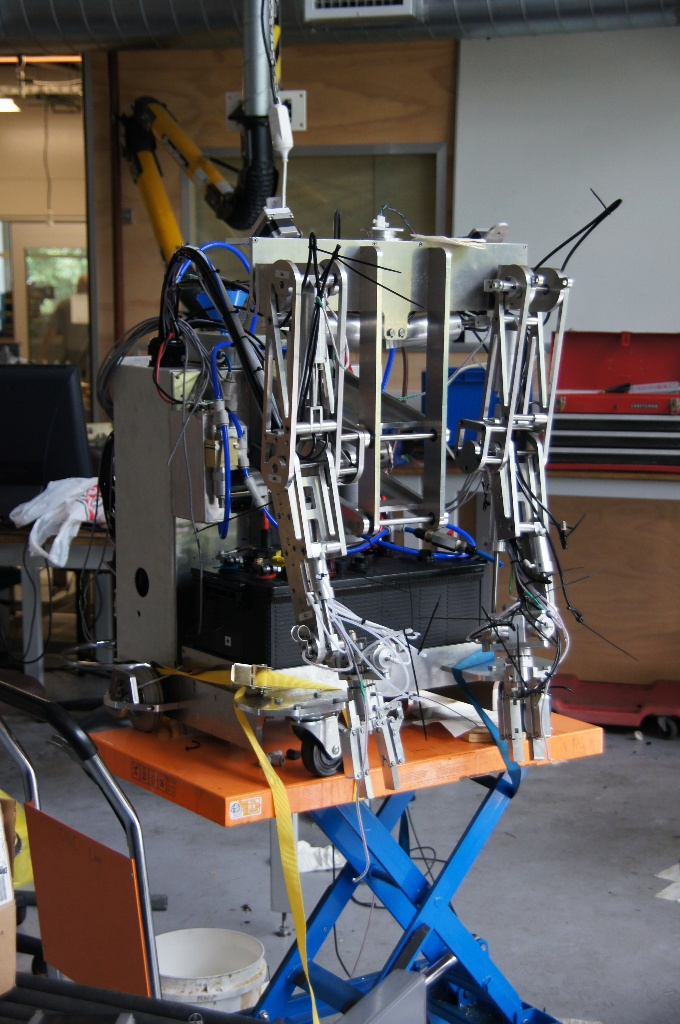
\includegraphics[width=0.75\linewidth]{images/junior}
\caption{Junior en cours de montage}
\end{figure}
\end{minipage}
&
\begin{minipage}{0.6\linewidth}
\begin{table}[h]
	\begin{center}
		\begin{tabular}{|c|c|}
		\hline
		%\multicolumn{2}{|c|}{Caract\'eristiques}\\
		%\hline
		Hauteur & $\sim~95~cm$\\
		Largeur & $\sim~65~cm$\\
		Longueur & $\sim~80~cm$\\
		Poids & $\sim~100~kg$\\
		Pression maximale & $\sim~10~bars$\\
		Charge effective & $\sim~30~kg$\\
		Vitesse de d\'eplacement & $inconnue$\\
		\hline
		\end{tabular}
	\end{center}
	\caption{Caract\'eristiques de Junior}
\end{table}
\end{minipage}
\end{tabular}
\end{center}
\end{frame}

\subsection{Matériel}
\begin{frame}
\begin{center}
\begin{figure}
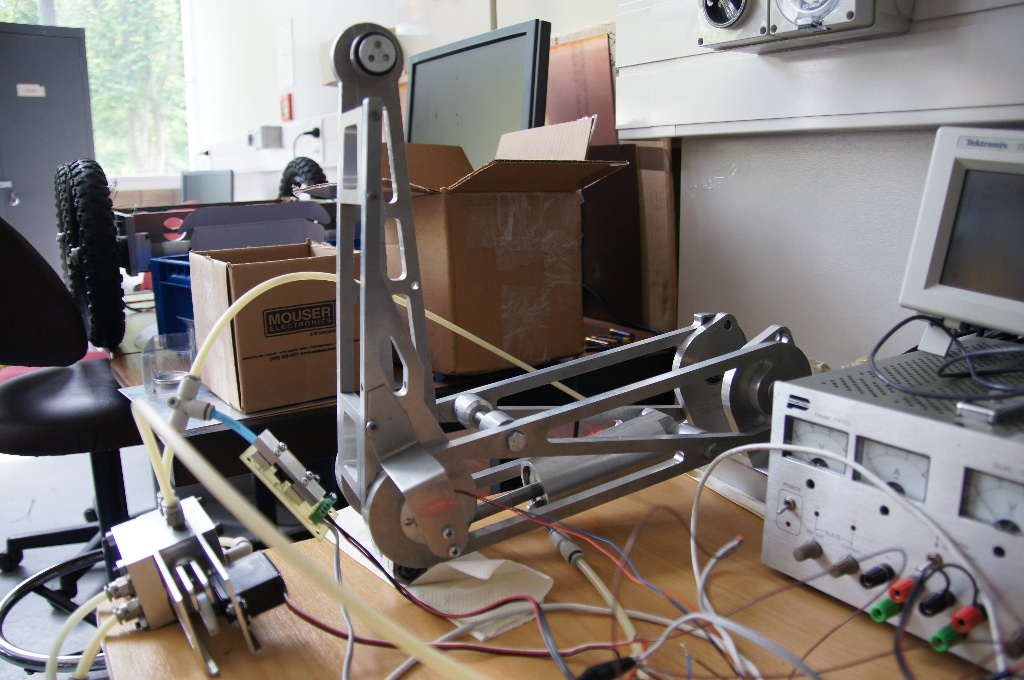
\includegraphics[width=0.75\linewidth]{images/bras}
\caption{Bras du robot pour les expériences}
\end{figure}
\end{center}
\end{frame}

\subsection{Résultats}
\begin{frame}
\begin{figure}
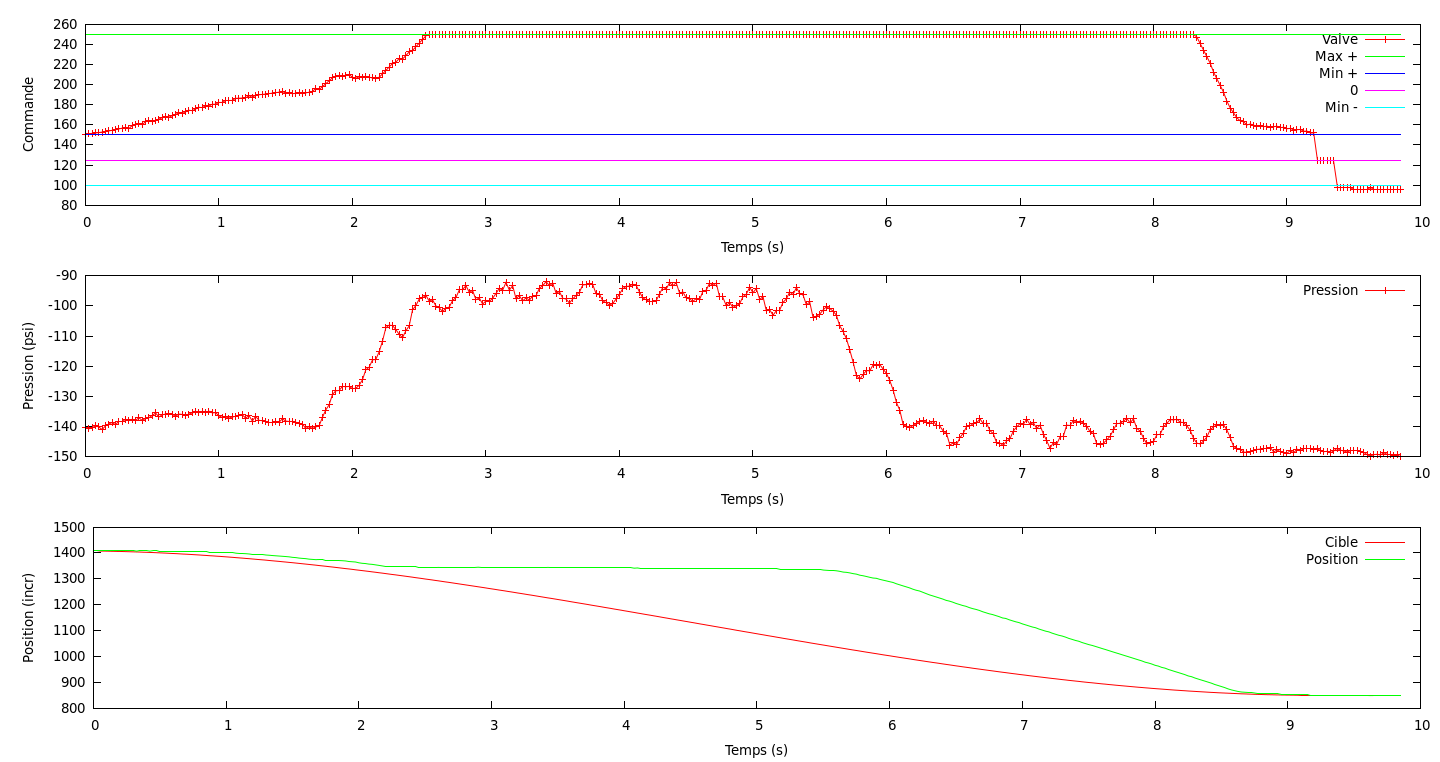
\includegraphics[width=1.05\linewidth]{images/stop}
\caption{Expérience de blocage du bras}
\end{figure}
\end{frame}

\section{Conclusion}
\subsection{Nouvelle-Zélande}
\begin{frame}
\begin{itemize}
\item A l'université
\begin{itemize}
\item Changement de sujet à l'arrivée
\item Problèmes de communication
\item Qualité des codes-sources fournis
\item Difficulté d'accès au matériel
\end{itemize}
\vspace{3mm}
\item En dehors de l'université
\begin{itemize}
\item Paysages magnifiques
\item Nourriture classique
\item Mode de vie étudiante inquiétant
\end{itemize}
\end{itemize}
\vspace{3mm}
\begin{itemize}
\item Points noirs
\begin{itemize}
\item \'Ecologie
\item Villes mortes
\item Insécurité/Gangs
\end{itemize}
\end{itemize}
\end{frame}

%\subsection*{Générale}
%\begin{frame}

%\end{frame}

\subsection{Conclusion Générale}
\begin{frame}
  \begin{itemize}
  \item Travaux de recherche
    \begin{itemize}
    \item Intérêts pour la recherche
    \item Difficultés rencontrées
    \item Publications
   \end{itemize}
   \vspace{3mm}
  \item Programmation
    \begin{itemize}
    \item Packaging
    \item Partage de code-source
    \item Apprentissage de langages
    \end{itemize}
%  \item Poursuite du projet
%    \begin{itemize}
%    \item Applications
%    \item Limites
%    \end{itemize}
\vspace{3mm}
\item Vie à l'étranger

  \end{itemize}
\end{frame}

\subsection{Discussion}
\begin{frame}
  \begin{center}
    \textit{Merci pour votre attention.}\\
    \huge{Avez-vous des questions ?}
  \end{center}
\end{frame}


\end{document}  
